Die wichtige verbleibende Frage besteht nun darin zu entscheiden, wann ein B\"undel trivial ist. F\"ur Vektorb\"undel \"uber Sph\"aren ist dies etwas einfacher als f\"ur beliebige andere R\"aume. Sei \(\xi\colon E\to\mathbb{S}^{k+1}\) ein orientiertes Vektorb\"undel vom Rang \(n\). Schreibe \({\mathbb{S}^{k+1}=H_1\cup H_2}\) als Vereinigung der oberen und unteren Hemisph\"are. Beachte hierbei \({H_1\cap H_2=\mathbb{S}^k}\). Da die \(H_i\) kontrahierbar sind, sind die Vektorb\"undel \(E|_{H_i}\) jeweils trivial. Seien
\[h_i\colon E|_{H_i}\to H_i\times\mathbb{R}^n\]
Trivialisierungen. Dann existiert eine Funktion \(h_{\xi}\colon\mathbb{S}^k\to\operatorname{GL}^+(n)\), sodass f\"ur alle \(x\in\mathbb{S}^k\) und \(y\in\mathbb{R}^n\)
\[h_2^{\phantom{}}h_1^{-1}(x,y)=(x,h_{\xi}(x)\cdot y)\]
gilt. Bezeichne diese Funktion \(h_{\xi}\) als \textbf{Kupplungsfunktion} (engl. Clutching-Func\-tion) von \(\pi\). Umgekehrt kann zu einer beliebigen Funktion \(f\colon\mathbb{S}^k\to\operatorname{GL}^+(n)\) ein orientiertes Vektorb\"undel \"uber \(\mathbb{S}^{k+1}\) gebildet werden, indem zwei triviale B\"undel \"uber den \(H_i\) mithilfe von \(f\) verklebt werden. Setze also
\[\left(H_1\times\mathbb{R}^n\sqcup H_2\times\mathbb{R}^n\right)/\left(\forall x\in\mathbb{S}^k\colon(x,y)\sim(x,f(x)\cdot y)\right)\]
mit der naheliegenden Projektion. Es l\"asst sich zeigen, dass homotope Kupplungsfunktionen mit orientiert isomorphen Vektorb\"undeln korrespondieren, sodass die Isomorphie
\begin{equation}
    \operatorname{Vekt}_n^+(\mathbb{S}^{k+1})\cong\left[\mathbb{S}^k,\operatorname{GL}^+(n)\right]\cong\pi_k\left(\operatorname{GL}^+(n)\right)\cong\pi_k\left(\operatorname{SO}(n)\right)
\end{equation}
gilt. Siehe zum Beispiel \cite{knapp2013vektorbuendel} Satz 3.1.11. Insbesondere ist ein Vektorb\"undel genau dann trivial, wenn die Kupplungsfunktion nullhomotop ist.

\begin{example}[M\"obius-Band]
    Das anschaulichste Beispiel einer nicht trivialen Kupplungsfunktion ist das (offene) M\"o\-bius\-band, auch wenn dieses nicht orientierbar ist und somit streng genommen nicht unter die obere Definition f\"allt. Hierbei werden zwei triviale Vektorb\"undel \(\underline{\mathbb{R}}\) \"uber \(\mathbb{D}^1\) entlang \(\partial\mathbb{D}^1=\mathbb{S}^0\) verklebt. Die Kupplungsfunktion ist dabei
    \[\phi\colon\mathbb{S}^0\to\operatorname{O}(1),\,x\mapsto\begin{cases}
        \mathbbm{1} & x=1\\
        -\mathbbm{1} & x=-1
    \end{cases}\]
    also nicht nullhomotop, sodass das B\"undel nicht trivial ist. 
    \[\mathbb{M}:=\left(\mathbb{D}\times\mathbb{R}\sqcup\mathbb{D}\times\mathbb{R}\right)/\left(\forall x\in\mathbb{S}^0\times\mathbb{R}\colon(x,y)_1\sim(x,\phi(x)\cdot y)_2\right)\,.\]
    Beachte, dass dieses B\"undel \textbf{nicht} orientierbar ist. Dies ver\"andert die Diskussion der Kupplungsfunktionen, da \(\operatorname{GL}\) im Gegensatz zu \(\operatorname{GL}^+\) zwei Zusammenhangskomponenten besitzt.
\end{example}

\begin{figure}
    \centering
    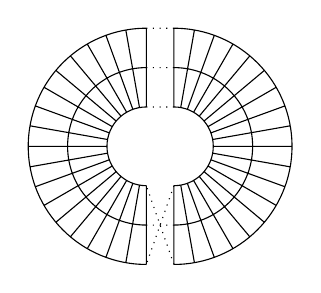
\begin{tikzpicture}[scale = 0.5]
        \begin{scope}[xshift = 0.35cm]
            \draw 
                (-90:1) arc (-90:90:1)
                (-90:2) arc (-90:90:2)
                (-90:3) arc (-90:90:3)
            \foreach\i in {-90,-80, ..., 90} {
                (\i:2) +(\i:-1) -- +(\i:1)
            };
        \end{scope}
        
        \begin{scope}[xshift = -0.35cm]
            \draw 
                (90:1) arc (90:270:1)
                (90:2) arc (90:270:2)
                (90:3) arc (90:270:3)
            \foreach\i in {90, 100, ..., 270} {
                (\i:2) +(\i:-1) -- +(\i:1)
            };
        \end{scope}
        \draw [dotted] 
            (0.35, 3) -- (-0.35, 3)
            (0.35, 2) -- (-0.35, 2)
            (0.35, 1) -- (-0.35, 1)
            (0.35, -1) -- (-0.35, -3)
            (0.35, -2) -- (-0.35, -2)
            (0.35, -3) -- (-0.35, -1)
            ;
    \end{tikzpicture}
    \caption{Das M\"obius-Band als nicht-triviales Vektorb\"undel \"uber der \(1\)-Sph\"are. Beachte, dass dieses nicht orientiert ist.}
\end{figure}